% !TeX spellcheck = en_GB
\documentclass[11pt]{article} 	% Set font size and document type

% Packages and settings
\usepackage[letterpaper, margin=1in]{geometry}	% Set page margins
\linespread{1.25}								% Equivalent to 1.5 spacing

\usepackage{float}
\usepackage{graphicx}
\usepackage{amsmath}
\usepackage{multicol}
\usepackage{multirow}
\usepackage{url}
\usepackage{placeins}
\usepackage{float}
\usepackage[acronym, nomain, nonumberlist]{glossaries}
\usepackage{verbatim}
\usepackage[binary-units=true]{siunitx}
\usepackage{listings}
\usepackage{subcaption}
\usepackage{wrapfig,lipsum,booktabs} 	% Get external packages
\title{SAVI Progress Report}


\author{
	Babak Esfandiari\\
	\texttt{babak@sce.carleton.ca}
	\and
	Gabriel Wainer\\
	\texttt{Gabriel.Wainer@sce.carleton.ca}
	\and
	Alan Davoust\\
	\texttt{alandavoust@gmail.com}
	\and
	Cristina Ruiz\\ 
	\texttt{cristinaruizmartin@sce.carleton.ca}
	\and	
	Patrick Gavigan\\
	\texttt{patrickgavigan@sce.carleton.ca}
	\and
	Guillermo Trabes\\
	\texttt{guillermotrabes@gmail.com}
}

\date{31 December 2018}	% Define metadata
% !TeX spellcheck = en_GB

\newacronym{BDI}{BDI}{Belief–Desire–Intention}
\newacronym{DEVS}{DEVS}{Discrete Event System Specification}

	% Define the acronyms
\renewcommand{\glossarysection}[2][]{}
\makeglossaries

\begin{document}
	% !TeX spellcheck = en_GB
% Front matter

\maketitle
\section*{Executive Summary}\label{sec:ExecutiveSummary}
This is the executive summary.
\addcontentsline{toc}{section}{Executive Summary}
\tableofcontents
\listoffigures
\listoftables
\pagebreak			% Insert front matter
	
	\FloatBarrier
\section{Scope and Purpose} \label{sec:ScopeAndPurpose}
\FloatBarrier

This is the scope and purpose section
	\FloatBarrier
\section{Background} \label{sec:Background}
\FloatBarrier

This is the background. It should introduce the concept of \gls{DEVS} and \gls{BDI} as implemented in Jason \cite{JasonBook}.

	\FloatBarrier
\section{Progress} \label{sec:Progress}
\FloatBarrier

This section discusses the progress to date. This will likely involve discussing figure \ref{fig:IntegrationOfJasonAndProcessing} and figure \ref{fig:RobotModelClassDiagram}, although that may go to a separate section on the implementation of the project.

\begin{figure}[!htbp]
	\begin{center}
		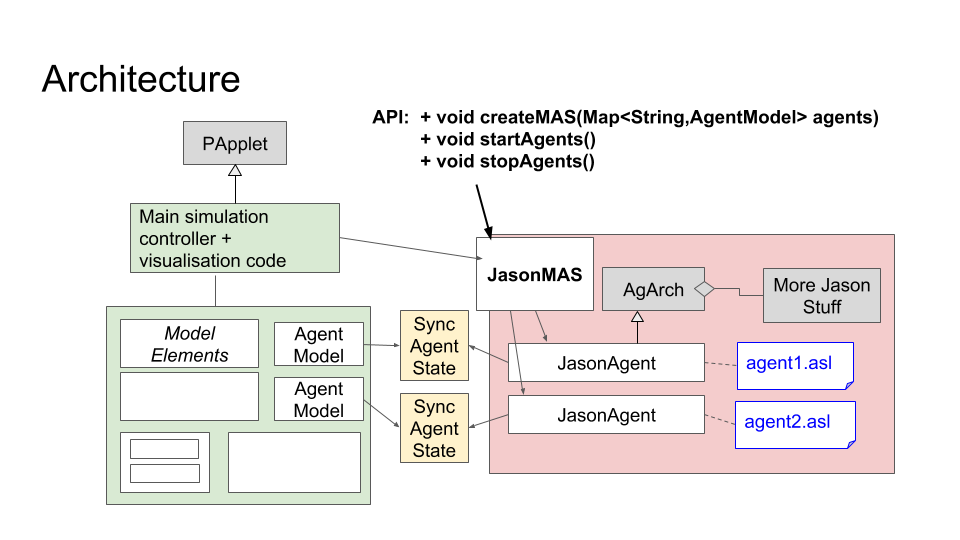
\includegraphics[width=0.6\textwidth,keepaspectratio]{Figures/jasonProcessingIntegration.png}
		\caption{Integration of Jason and Processing.}
		\label{fig:IntegrationOfJasonAndProcessing}
	\end{center}
\end{figure}

\begin{figure}[!htbp]
	\begin{center}
		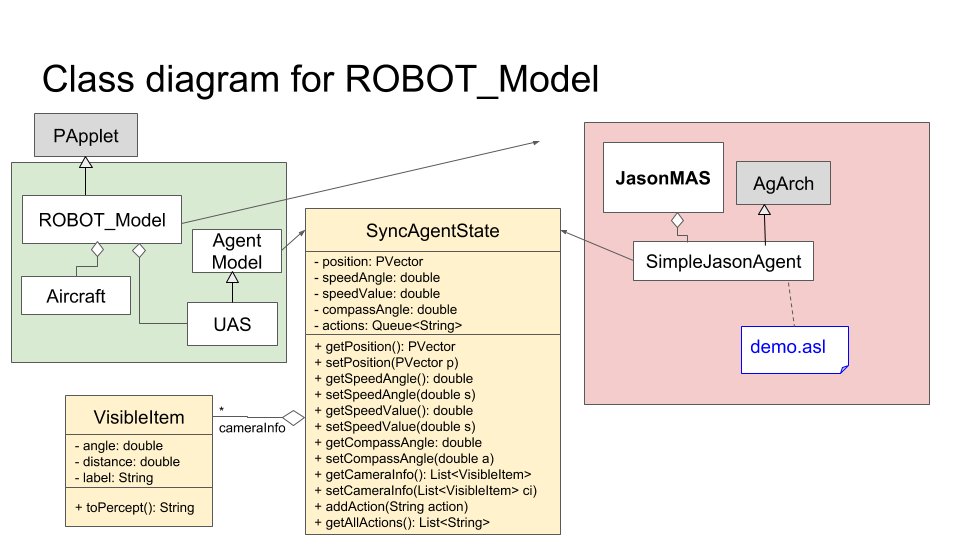
\includegraphics[width=0.6\textwidth,keepaspectratio]{Figures/robotModelClassDiagram.png}
		\caption{Robot model class diagram.}
		\label{fig:RobotModelClassDiagram}
	\end{center}
\end{figure}
	\FloatBarrier
\section{Remaining Work}\label{sec:RemainingWork}
\FloatBarrier

What else is there to do? Discuss the schedule?

% Generated using http://www.tablesgenerator.com/#

\begin{table}[!htbp]
	\centering
	\caption{An example table}
	\label{AnExampleTable}
	\begin{tabular}{|c|c|c|}
		\hline
		Heading & \begin{tabular}[c]{@{}c@{}}Another\\ Heading\end{tabular} & Something   \\ \hline
		Some    & interesting                                               & information \\ \hline
		that    & we want to                                                & share       \\ \hline
	\end{tabular}
\end{table}
	\FloatBarrier
\section{Results} \label{sec:Results}
\FloatBarrier

Results so far or projected go here.

\subsection{Example sub section}
Say something here.
	\FloatBarrier
\section{Discussion} \label{sec:Discussion}
\FloatBarrier

Discussion section is here.
	\FloatBarrier
\section{Conclusion} \label{sec:Conclusion}
\FloatBarrier

Conclude here. 

	\FloatBarrier
	\section*{List of Acronyms}\label{sec:ListOfAcronyms}
	\begin{multicols}{2}
		\printglossary[type=\acronymtype]
	\end{multicols}

	\bibliography{refs}
	\bibliographystyle{ieeetr}

\end{document}
